\documentclass[aspectratio=169, 11pt]{beamer}
\usepackage{multicol}
\usepackage{graphicx}
\usepackage{hyperref}
\usepackage{booktabs}
\usepackage{array}
\usepackage{amsmath}
\hypersetup{
    colorlinks=true,
    linkcolor=blue,
    urlcolor=blue,
    citecolor=blue
}

% --- Minimalist Theme Settings ---
\usetheme{default}
\useinnertheme{circles} % Clean bullet points
\useoutertheme{miniframes} % Small header dots
\setbeamertemplate{navigation symbols}{} % Remove navigation bar
\addtobeamertemplate{navigation symbols}{}{%
  \usebeamerfont{footline}%
  \usebeamercolor[fg]{footline}%
  \hspace{1em}%
  \insertframenumber/\inserttotalframenumber
}

% --- Presentation Metadata ---
\title{MSBGen}
\author{Devadatta M. Pokharanakar}
\institute{MTech DS, IIT PKD}
\date{November 07, 2026}

\begin{document}

% \begin{frame}
%     \titlepage
% \end{frame}

\begin{frame}
    \begin{center}
        {\LARGE\bfseries\usebeamercolor[fg]{structure} MSBGen}
        
        \vfill
        {\normalsize Generative Image Reconstruction from
        Most-Significant Bitplanes}

        \vfill
        {\large\bfseries Devadatta M. Pokharanakar}
    \end{center}
\end{frame}

\begin{frame}{Motivation: Can We Generate What We Don't Transmit?}
    \begin{itemize}
        \item Conventional 8-bit images require 8 bits/pixel per channel.
        \item The Most Significant Bit (MSB) contains coarse intensity and structural information.
        \item Can we transmit only the MSB and generate the remaining information at the receiver?
    \end{itemize}

    \vspace{-0.9cm}
    \begin{center}
        \[
            I = 128B_7 + 64B_6 + \cdots + B_0
        \]
        \[
            \underbrace{I_{\text{top}}=128B_7}_{\text{Transmitted}}
            \qquad
            \underbrace{R=I-128B_7}_{\text{Missing information}}
        \]
        \[
            \boxed{\hat I = 128B_7 + \hat R}
        \]
    \end{center}

    \vspace{-0.3cm}
    \begin{block}{Core Research Question}
        Can conditional generative models reconstruct a perceptually useful full image from an extremely limited representation?
    \end{block}

    \textbf{Key challenge:} Multiple original images can share the same MSB plane. This is an inherently one-to-many reconstruction problem.

    \vspace{0.1cm}
    \footnotesize
    For RGB, transmitting one MSB per channel corresponds to 3 binary planes/pixel before entropy coding.
\end{frame}

\begin{frame}{Existing Research}
\small
\begin{itemize}
    \item \textbf{Punnappurath \& Brown (2020) -- Bitplane-wise Bit-depth Recovery}~[\ref{ref:bitdepth2020}]
    \begin{itemize}
        \item Uses a CNN to predict missing lower bitplanes sequentially.
        \item Focuses on recovering bit depth from partially available bitplanes.
    \end{itemize}

    \vspace{0.2cm}
    \item \textbf{Chang et al. (2021) -- Progressive Medical Image Transmission}~[\ref{chang2021}]
    \begin{itemize}
        \item Uses a bank of GANs for progressive medical image transmission.
        \item Generates image refinements at successive transmission stages.
    \end{itemize}

    \vspace{0.2cm}
    \item \textbf{Han et al. (2025) -- Bit Plane Decomposition for INR}~[\ref{han2025}]
    \begin{itemize}
        \item Uses bitplane decomposition within an implicit neural representation.
        \item Aims at lossless image representation.
    \end{itemize}

\end{itemize}
\end{frame}

\begin{frame}{Research Gap}
\small
\begin{itemize}
    \item Existing bitplane-based methods primarily focus on:
    \begin{itemize}
        \item Sequential recovery of missing lower bitplanes.
        \item Lossless representation using bitplane decomposition.
        \item Progressive image transmission through multiple stages.
    \end{itemize}

    \vspace{0.3cm}
    \item \textbf{What is less explored?}
    \begin{itemize}
        \item Direct reconstruction of the complete image using only the top $k$ most significant bitplanes.
        \item Learning the missing image information as a residual rather than explicitly predicting each lower bitplane.
        \item Comparing regression-based and generative approaches for this task.
    \end{itemize}

    \vspace{0.3cm}
    \item \textbf{My objective:} Given the top $k$ MSB planes, reconstruct a visually plausible full 8-bit grayscale or RGB image.
\end{itemize}
\end{frame}

\begin{frame}{From Regression to Generative Models}
\small
\textbf{1. Regression-based reconstruction}

\begin{itemize}
    \item CNN, U-Net and residual U-Net models directly predict the missing image residual from the available MSB planes.
    \item They learn a deterministic mapping from the input bitplanes to the reconstructed image.
    \item These models provide strong pixel-level reconstruction baselines.
\end{itemize}

\vspace{0.3cm}
\textbf{2. Why explore generative models?}

\begin{itemize}
    \item Multiple plausible images may correspond to the same limited MSB information.
    \item A deterministic prediction may not capture the uncertainty in the missing details.
    \item Generative models allow the reconstruction of diverse, plausible high-frequency details.
\end{itemize}
\end{frame}

\begin{frame}{From Regression to Generative Models}
\small
\textbf{Generative approaches explored}

\begin{itemize}
    \item \textbf{Conditional Diffusion:}
    Iteratively denoises a residual conditioned on the available MSB planes.

    \item \textbf{Flow Matching:}
    Learns a continuous transformation from noise to a plausible residual.

    \item \textbf{Conditional Normalizing Flow:}
    Learns an invertible mapping to model the conditional residual distribution.
\end{itemize}

\vspace{0.3cm}
\textbf{Hybrid approach}

\begin{itemize}
    \item Residual U-Net provides an initial reconstruction.
    \item Flow matching models a residual correction.
    \item Diffusion further refines the generated result.
\end{itemize}

\vspace{0.2cm}
\centering
\textbf{Goal: Combine accurate reconstruction with perceptually plausible details.}
\end{frame}

\begin{frame}{Results: RGB Kodak Benchmark}
    \small
    \textbf{Experimental setup}
    \begin{itemize}
        \item Training: 800 RGB DIV2K; Evaluation: 24 RGB Kodak images.
        \item $k$ = number of retained MSB planes per channel.
        \item Compare sequential bitplane CNN (D4) against the proposed three-stage hybrid.
    \end{itemize}

    \vspace{0.1cm}
    \textbf{Quantitative comparison}
    \begin{table}
        \centering
        \setlength{\tabcolsep}{5pt}
        \begin{tabular}{c cc cc cc}
            \toprule
            & \multicolumn{2}{c}{\textbf{PSNR (dB)} $\uparrow$}
            & \multicolumn{2}{c}{\textbf{LPIPS} $\downarrow$}
            & \multicolumn{2}{c}{\textbf{KID ($\times 10^3$)} $\downarrow$}
            \\
            \cmidrule(lr){2-3}
            \cmidrule(lr){4-5}
            \cmidrule(lr){6-7}
            $k$ & D4 & Hybrid & D4 & Hybrid & D4 & Hybrid \\
            \midrule
            1 & 18.40 & \textbf{18.56} & 0.4481 & \textbf{0.4223} & 87.81 & \textbf{53.35} \\

            2 & \textbf{27.00} & 26.48 & 0.2367 & \textbf{0.1898} & 50.51 & \textbf{18.13} \\

            3 & \textbf{33.89} & 32.52 & 0.0964 & \textbf{0.0772} & 21.43 & \textbf{6.12} \\
            \bottomrule
        \end{tabular}
    \end{table}

    \vspace{0.2cm}
    \begin{itemize}
        \item Sequential bitplane CNN achieves higher PSNR at $k=2,3$.
        \item Hybrid consistently improves LPIPS and KID across all three bit-depth settings.
        \item Hybrid preserves transmitted MSBs exactly (MSB consistency = 1).
    \end{itemize}

    \vspace{0.1cm}
    \footnotesize
    Results are means over 24 images. Lower LPIPS and KID indicate better perceptual similarity and distributional quality, respectively. Single training runs; not a multi-seed benchmark.
\end{frame}

\begin{frame}[plain]
    \vspace*{-0.35cm}
    % \hspace*{-0.5cm}
    \centering
    \small
    \begin{columns}[T,onlytextwidth]
        \column{0.333\textwidth}
        \centering
        \textbf{Original Image}

        \vspace{0.15cm}
        
\includegraphics[width=\linewidth,height=0.80\textheight,keepaspectratio]{images/original.png}

        \vspace{0.15cm}
        \footnotesize Full 8-bit image

        \column{0.333\textwidth}
        \centering
        \textbf{First MSB Plane}

        \vspace{0.15cm}
        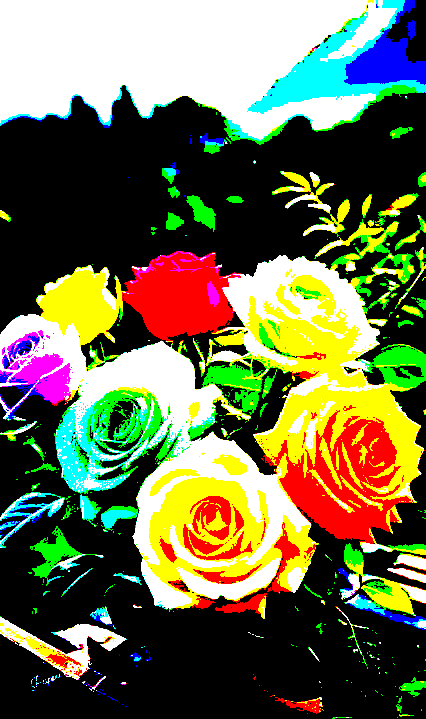
\includegraphics[width=\linewidth,height=0.80\textheight,keepaspectratio]{images/msb_binary.png}

        \vspace{0.15cm}
        \footnotesize Binary representation of the first MSB

        \column{0.333\textwidth}
        \centering
        \textbf{MSB-only Image}

        \vspace{0.15cm}
        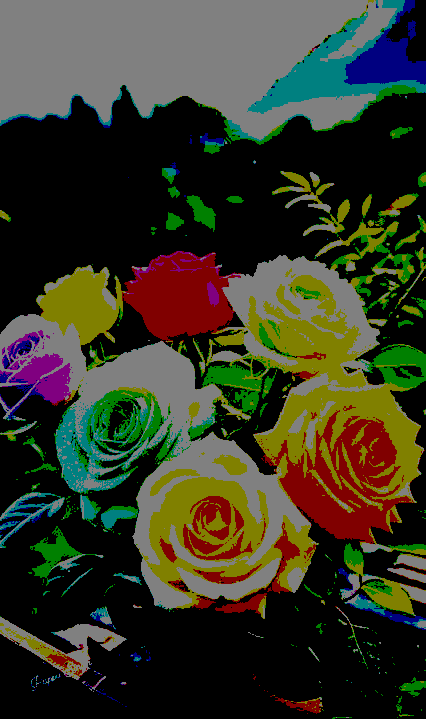
\includegraphics[width=\linewidth,height=0.80\textheight,keepaspectratio]{images/msb_reconstructed.png}

        \vspace{0.15cm}
        \footnotesize First MSB retained; all other planes set to zero
    \end{columns}
\end{frame}

\newcommand{\PortraitResult}[8]{%
    \begin{minipage}[t]{0.3\textwidth}
        \centering
        {\footnotesize\bfseries #1}\vspace{0.03cm}

        \includegraphics[
            width=0.90\linewidth,
            height=0.80\textheight,
            keepaspectratio
        ]{#2}

        \vspace{0.02cm}

        {\fontsize{5}{5.5}\selectfont
        \begin{tabular}{@{}lr@{}}
            PSNR (dB) $\uparrow$ & #3 \\
            SSIM $\uparrow$ & #4 \\
            LPIPS $\downarrow$ & #5 \\
            DISTS $\downarrow$ & #6 \\
            MAE $\downarrow$ & #7 \\
            Time (s) $\downarrow$ & #8 \\
        \end{tabular}}
    \end{minipage}%
}

\begin{frame}[plain]
    \vspace*{-0.35cm}
    \hspace*{-0.5cm}
    \makebox[\paperwidth][c]{%
        \PortraitResult
            {U-Net}
            {images/unet.png}
            {18.01}{0.65}{0.3571}{0.2273}{26.80}{0.126}
        % \hfill
        \PortraitResult
            {Flow Matching}
            {images/flowmatching.png}
            {18.07}{0.6323}{0.3461}{0.1851}{26.03}{0.606}
        % \hfill
        \PortraitResult
            {Diffusion}
            {images/diffusion.png}
            {17.87}{0.6287}{0.3403}{0.1924}{26.45}{0.605}
    }
\end{frame}

\begin{frame}[plain]
    \vspace*{-0.35cm}
    \hspace*{-0.5cm}
    \makebox[\paperwidth][c]{%
        \PortraitResult
            {U-Net Hybrid}
            {images/hybrid.png}
            {18.04}{0.6423}{0.3467}{0.1844}{26.11}{1.086}
        % \hfill
        \PortraitResult
            {ViT Hybrid}
            {images/vit_hybrid.png}
            {17.33}{0.6268}{0.3557}{0.2030}{27.28}{1.365}
        % \hfill
        \PortraitResult
            {Bitdepth D4}
            {images/bitdepth_d4.png}
            {18.03}{0.6574}{0.3445}{0.1781}{26.26}{2.001}
    }
\end{frame}

\begin{frame}{Conclusion and Takeaways}
    \begin{enumerate}
        \item \textbf{Feasibility:} Useful full-image reconstruction is possible even when only a small number of MSB planes are retained.

        \vspace{0.2cm}
        \item \textbf{Hybrid modeling:} Combining deterministic regression with flow matching and diffusion improves perceptual metrics over standalone bitplane CNN recovery.

        \vspace{0.2cm}
        \item \textbf{Perception vs. distortion:} No single method wins across all metrics. Better perceptual similarity can come with a small PSNR trade-off.

        \vspace{0.2cm}
        \item \textbf{Potential application:} Generative reconstruction offers a direction towards extremely low-bitrate image communication.
    \end{enumerate}

    \vspace{0.35cm}
    \begin{block}{Current Limitations}
        Evaluation is based on a single training run and 24 Kodak test images. Multiple seeds, additional datasets, actual entropy-coded bitrate measurements and inference scaling remain important next steps.
    \end{block}

    \vspace{0.2cm}
    \begin{center}
        \Large\bfseries Thank You!
    \end{center}

\end{frame}

\begin{frame}{References}
    \small
    \begin{enumerate}
        \item Punnappurath, A. and Brown, M. S. (2020). \textit{A Little Bit More: Bitplane-Wise Bit-Depth Recovery.} IEEE TPAMI. \href{https://arxiv.org/abs/2005.01091}{arXiv:2005.01091}\label{ref:bitdepth2020}
        
        \vspace{0.2cm}
        \item Chang et al. (2021). \textit{Progressive Transmission of Medical Images via a Bank of GANs.} \href{https://doi.org/10.1155/2021/9917545}{DOI: 10.1155/2021/9917545}\label{chang2021}

        \vspace{0.2cm}
        \item Han et al. (2025). \textit{Towards Lossless Implicit Neural Representation via Bit Plane Decomposition.} \href{https://doi.org/10.48550/arXiv.2502.21001}{arXiv:2502.21001}\label{han2025}

    \end{enumerate}
    \vfill
    My code is available at: \url{https://github.com/DevadattaP/MSBGen}
\end{frame}

\end{document}
